\documentclass{article}

% if you need to pass options to natbib, use, e.g.:
%     \PassOptionsToPackage{numbers, compress}{natbib}
% before loading neurips_2020

% ready for submission
\usepackage[final]{neurips_2020}

% to compile a preprint version, e.g., for submission to arXiv, add add the
% [preprint] option:
%     \usepackage[preprint]{neurips_2020}

% to compile a camera-ready version, add the [final] option, e.g.:
%     \usepackage[final]{neurips_2020}

% to avoid loading the natbib package, add option nonatbib:
%\usepackage[nonatbib]{neurips_2020}

\usepackage[utf8]{inputenc} % allow utf-8 input
\usepackage[T1]{fontenc}    % use 8-bit T1 fonts
\usepackage{hyperref}       % hyperlinks
\usepackage{url}            % simple URL typesetting
\usepackage{booktabs}       % professional-quality tables
\usepackage{amsfonts}       % blackboard math symbols
\usepackage{nicefrac}       % compact symbols for 1/2, etc.
\usepackage{microtype}      % microtypography

\usepackage{graphicx}
\graphicspath{ {./figs/} }

\title{Randomized Overdrive Neural Networks}

% The \author macro works with any number of authors. There are two commands
% used to separate the names and addresses of multiple authors: \And and \AND.
%
% Using \And between authors leaves it to LaTeX to determine where to break the
% lines. Using \AND forces a line break at that point. So, if LaTeX puts 3 of 4
% authors names on the first line, and the last on the second line, try using
% \AND instead of \And before the third author name.

\author{%
  Christian J. ~Steinmetz \\
  Queen Mary University of London\\
  \texttt{c.j.steinmetz@qmul.ac.uk} \\
  \And
  Joshua D.~Reiss \\
  Queen Mary University of London \\
  \texttt{joshua.reiss@qmul.ac.uk} \\
}

\begin{document}

\maketitle

\begin{abstract}

By processing audio signals in the time-domain with randomly weighted temporal convolutional networks (TCNs),
we uncover a wide range of novel, yet controllable overdrive effects.
We find that architectural aspects, such as the depth of the network, 
the kernel size, the number of channels, the activation function, as well as the weight initialization, 
have a clear impact on the sonic character of the resultant effect, without the need for training. 
In practice, these effects range from relatively conventional overdrive effects,
to more extreme effects, as the receptive field grows, akin to a fusion of distortion, equalization, delay, and reverb.  
To enable use by musicians and producers, we provide a real-time plugin implementation.
This allows users to dynamically design networks, listening to the to the results in real-time.
We provide a demo, along with plugin builds at \url{https://ronn.ml}.

\end{abstract} 

% The TCN architecture can be viewed as a nonlinear waveshaper with memory
% equal to receptive field of the causal convolutional network. 

\section{Introduction}

Throughout the history of audio technology, engineers, circuit designers, 
and particularly guitarists, have searched for novel sonic effects as a result of clipping or distorting audio signals. 
These distortion effects were first discovered by pushing early guitar amplifiers beyond their operating range, 
or, in some cases, even from the accidental damage to amplifiers or speakers \cite{shepherd2003distortion}. 
These pursuits are a clear example of creators taking advantage of the limitations of their tools for creative effect.
Today, distortion effects are commonplace and have permeated most genres such as blues, jazz, rock, and metal, as well as modern pop and hip-hop styles.
Whether it be vacuum tubes, diodes, transistors, integrated circuits, or software-based digital models, 
it may appear as if nearly all the methods of generating distortion-based effects have been exhausted. 

Neural networks are far from new, and in fact they arose in the same era that blues guitarists began their experiments with distortion \cite{schmidhuber2015deep}.
Yet, with the emergence of modern deep learning approaches, which have demonstrated the ability to tackle many modeling tasks in the audio domain,
these methods have now been applied to the task of trying to mimic the characteristic distortion of famous amplifiers and distortion effects 
\cite{covert2013rnn, schmitz2018nonlinear, zhang2018lstm, damskagg2019distortion, martinez2019nonlinear}.
While these approaches have largely been successfully in this emulation task, the aim of our work deviates from these modeling approaches.
In a similar spirit to the guitarists using their amplifiers in a fashion unintended by their designers,
we propose the apparent abuse of temporal convolutional networks (TCNs) \cite{bai2018tcn} by utilizing randomly initialized networks 
to process, distort, and warp audio signals for creative effect. 

\section{Method}
\subsection{Architecture}

The TCN framework aims to outline a set of design choices ideal for various sequence modeling tasks, such as time domain audio signals. 
Casual convolutions are a core component, in which outputs are predicted considering only past values,
so information from the future does not "leak" into current predictions. 
Additionally, these networks are generally built to be fully convolutional, 
so they can process input signals of arbitrary length, and will produce an output signal with length proportional to the input length \cite{long2015fcn}.
With standard casual convolutions the receptive field grows linearly as the depth of the network increases, 
making it challenging to achieve models that are able to consider larger time contexts. 
To address this, the TCN incorporates dilated convolutions \cite{oord2016wavenet}, 
which inserts zeros within the taps of the convolutional kernels, effectively increasing the size of the kernel without additional computation. 
To increase the receptive field more rapidly, an exponentially decreasing dilation factor is generally applied at each layer in the network. 

With this framework it is easy to construct a randomly weighted network for audio signal processing.
Since the TCN enables the ability to produce any number of output channels, 
we setup the networks to produce a stereo output signal, given only a monophonic input signal, such as a guitar. 
In our listening, we found that this often produced interesting spatialized results. 

\subsection{Implementation}
For the real-time implementation, \texttt{ronn}, we utilize the JUCE framework\footnote{\url{https://github.com/juce-framework/JUCE}},
which enables us to create a VST/AU plugin that can easily run in popular digital audio workstations (DAWs).
In order to construct the TCN models, we utilize PyTorch \cite{pytorch}, which features a C++ API. 
This enabled us to develop our own parameterized neural network module class that can be instantiated within the main JUCE plugin.
By connecting this class with the user interface, the on-screen controls, as shown in Figure \ref{fig:ui},
can be used to dynamically construct new networks, generating new effects, all in a paradigm that allows for real-time interaction. 

There are some challenges in the implementation of the TCNs for real-time processing.
One such challenge arises from the reality that these models are fully convolutional,
yet the plugin paradigm requires that all processing within the plugin occurs on a block-by-block basis. 
This means that unlike other scenarios where the TCN may be employed, such as speech processing \cite{}, 
we do not have access to the entire signal. Instead, we see only small blocks of audio samples at a time (e.g. 512).
To address this, we construct a lookback buffer the size of the receptive field of the TCN. 
This buffer then stores all the past input samples to the model, which can then be passed for prediction, 
along with the new samples provided in the current block. 
In practice, we found that this method works quite well, and produces no perceivable discontinuities at the frame boundaries, 
but as to be expected, as the size of the receptive field increases, the computational load increases, 
causing the plugin to perform in less than real-time, when the receptive field becomes excessively larger ($\geq$ 4 seconds).

To address the significant computational overhead imposed by deeper models with large receptive field, 
we introduce the ability to swap traditional convolutions with depthwise convolutions \cite{howard2017mobilenets}.
These convolutions greatly reduce the number of parameters and computational overhead by convolving $K$ filters
with only a single input channel each. 
We found that by using depthwise convolutions we were able to run models with larger receptive fields in real-time on the CPU,
making a wider range of effects achieve on the general purpose hardware utilized my musicians and producers. 


\section{Discussion}

We propose the use of randomly weighted TCNs as complex, time-domain audio signal processing systems. 
We find that making adjustments to various architectural aspects results in the ability to generate a wide range of compelling sonic effects
that range from conventional distortion and overdrive, to .
Additionally, there appears to be a clear link between different aspects of the architecture and the kinds of effects generated, 
which enable a level of interpretable control over the generated effect. 
While deep networks pose a challenge for real-time implementation due to significant compute overhead, 
when constructed with the more computationally efficient depthwise convolutions,
we are able to provide a real-time implementation. 
This real-time plugin implementation enables the use of this set of effects within popular DAWs. 
With a simplified interface, musicians and producers without machine learning experience can easily take advantage of these effects.
While we have only investigated feedforward architectures, 
it reasons that we could achieve a wider range of effects with the addition of recurrence.

\section*{Broader Impact}
In this work we apply existing neural network approaches for processing audio signals in a creative context.
Since we do not utilize any training data in this process there is a relatively low . 
Potential biases in the processing of signals from , although such biases are not chosen intentionally, 
and simply reflect the underlying characteristics of these generated effects, 
which represent only a limited number of all possible audio effects. 

\bibliography{references}{}
\bibliographystyle{plain}

\newpage
\section*{Supplementary materials}

\begin{figure}[h] 
  \centering
  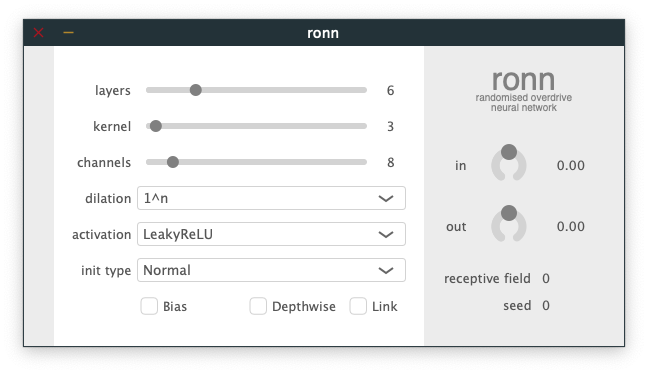
\includegraphics[width=0.8\textwidth]{ronn-vst-ui.png}  
  \caption{Real-time plugin user interface, featuring a series of sliders and selection boxes, 
  enabling users to dynamically construct various TCN architectures while listening to the results.}
  \label{fig:ui}
\end{figure}

\end{document}
